\documentclass[aspectratio=169,x11names]{beamer}
\usetheme{Pittsburgh}
\usepackage{xcolor}
\usepackage[utf8]{inputenc}
\usepackage[german]{babel}
\usepackage{amsmath}
\usepackage{amsfonts}
\usepackage{amssymb}
\usepackage{graphicx}
\usepackage{multicol}
\usepackage{wrapfig}
\usepackage{hyperref}

\author{Jonas Betzendahl}
\title{Machine Learning Science Slam}

\beamertemplatenavigationsymbolsempty 

% For Footnotes without markers on the slide
% https://tex.stackexchange.com/questions/30720/footnote-without-a-marker
\newcommand\blfootnote[1]{%
  \begingroup
  \renewcommand\thefootnote{}\footnote{#1}%
  \addtocounter{footnote}{-1}%
  \endgroup
}

\begin{document}

%------------------------------------------------------------------------------------
\section{Introduction}

\begin{frame}
\begin{center}
\Large \glqq Maschine Learning\grqq
\normalsize 

(And why that may be spookier than it sounds)
\bigskip\bigskip

\Large Jonas Betzendahl\\
\texttt{@lambdaTotoro}
\smallskip

\href{https://twitter.com/lambdatotoro}{
\includegraphics[scale=0.125]{images/twitter_logo.png}}
\href{https://github.com/jbetzend}{
\includegraphics[scale=0.125]{images/github_logo.png}}
\href{https://whispeer.de/en/user/jbetzend}{
\includegraphics[scale=0.125]{images/whispeer_logo.png}}
\end{center}
\end{frame}

%------------------------------------------------------------------------------------

\begin{frame}
\frametitle{Small Talk in Intelligent Systems}

\begin{multicols}{2}

The question I get asked most often:

\pause

\begin{center}
\glqq So\dots how long until the\\ killer robot apocalypse?\grqq
\end{center}

\columnbreak

\begin{center}

\includegraphics[height=0.7\textheight,keepaspectratio]{images/mtt.png} 
\end{center}

\end{multicols}

\end{frame}

\begin{frame}
\begin{center}

\includegraphics[width=\textwidth]{images/amazon-logo.jpg} 
\end{center}
\end{frame}

\begin{frame}
\begin{center}

\includegraphics[width=\textwidth]{images/amazon-one-wallet.jpg} 
\end{center}
\end{frame}

\begin{frame}
\begin{center}
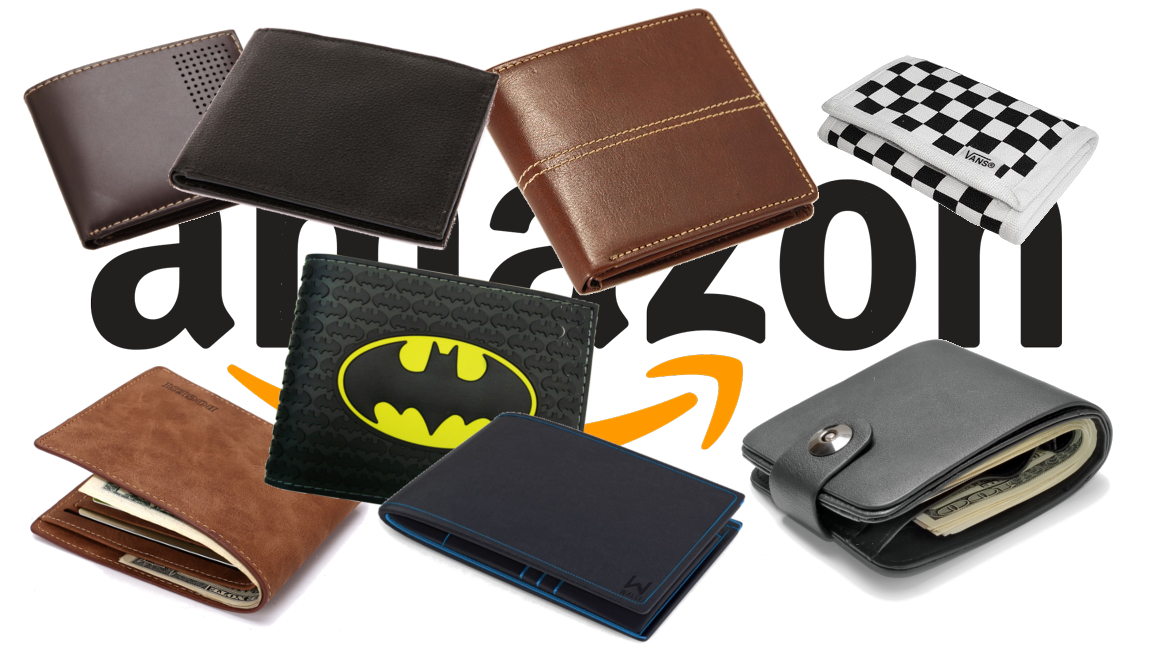
\includegraphics[width=\textwidth]{images/amazon-buncha-wallets.jpg} 
\end{center}
\end{frame}

%------------------------------------------------------------------------------------

\begin{frame}

\begin{center}
\dots at least that's how I \emph{used to} start my slams.
\pause\bigskip

We need to talk!
\end{center}

\end{frame}

\section{Die Vorteile von Maschinellem Lernen}

\begin{frame}
\begin{center}
\huge
Machine Learning's\\ Grand Accomplishments
\end{center}
\end{frame}

\begin{frame}

\begin{center}
Machine learning is very powerful and useful in principle\dots
\end{center}

\begin{center}
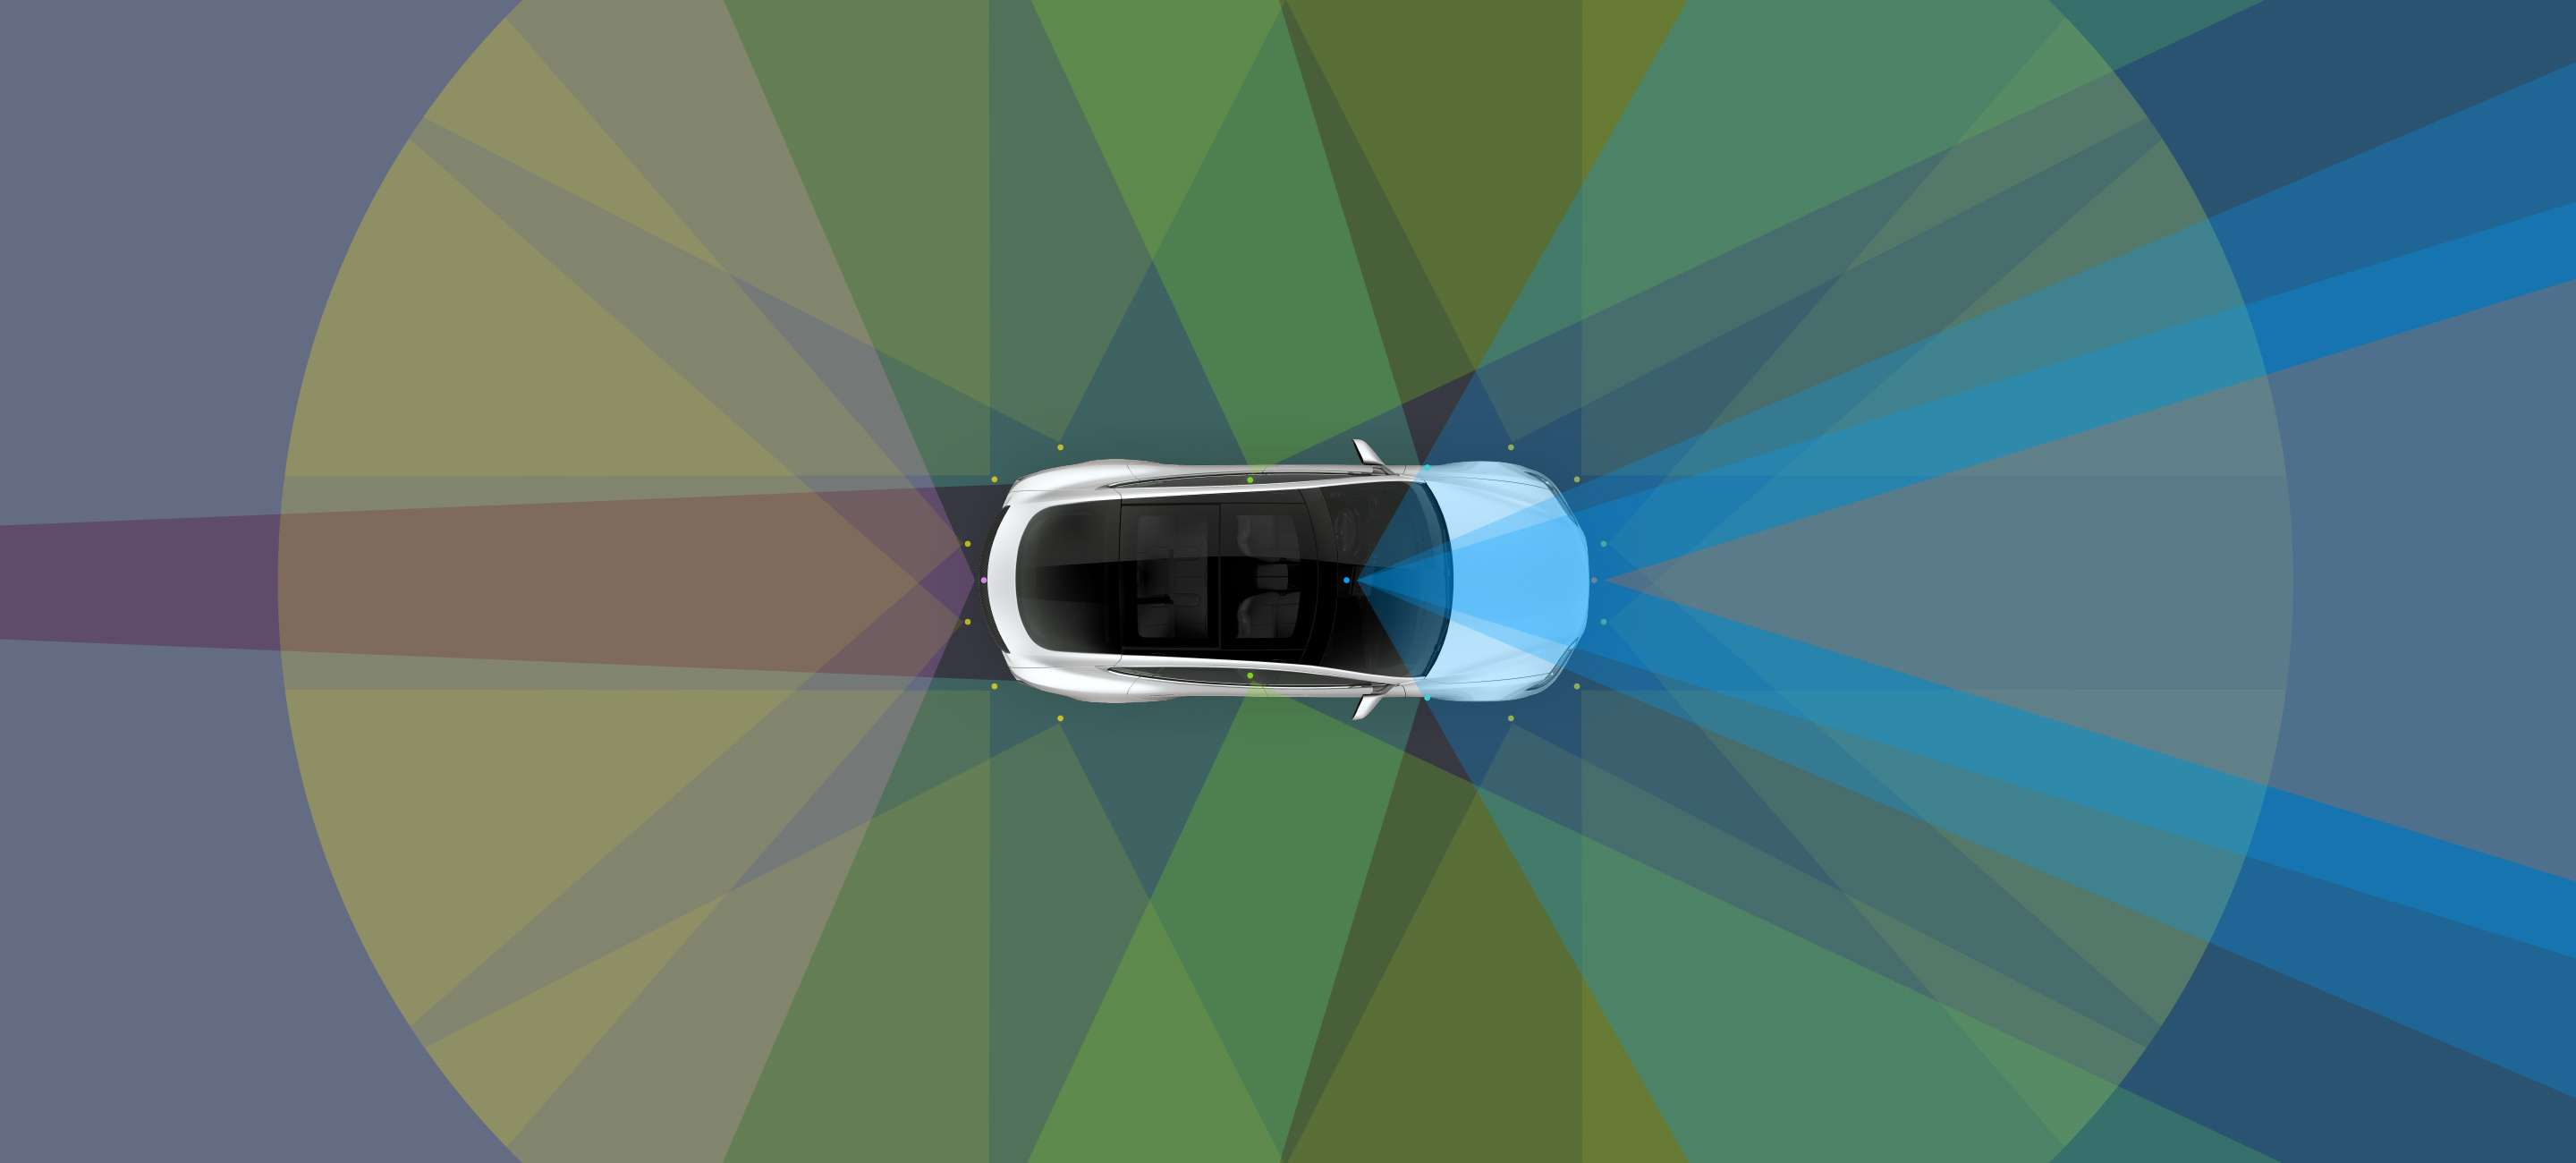
\includegraphics[width=.9\textwidth]{images/autopilotnew.jpg} 
\end{center}
\end{frame}

%------------------------------------------------------------------------------------

\section{Was ist Maschinelles Lernen?}

\begin{frame}
\begin{center}
\huge
Machine Learning\\ in a Nutshell
\end{center}
\end{frame}

\begin{frame}
\begin{center}
\Large Imitation is the highest form of flattery!
\medskip\medskip

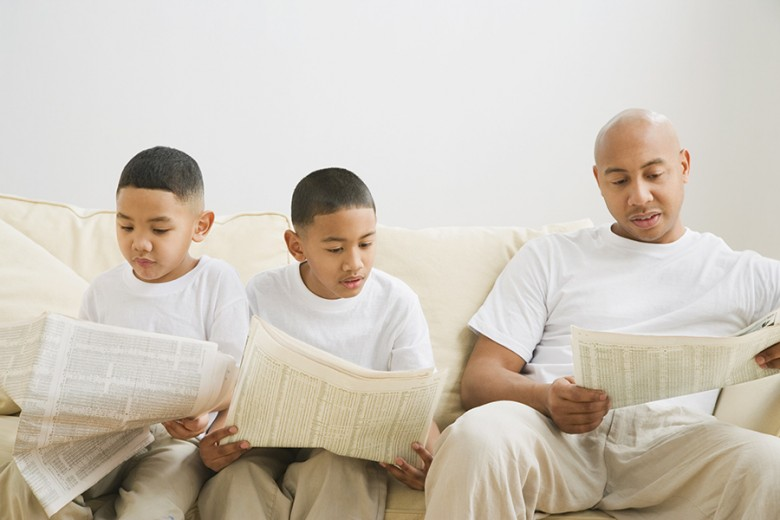
\includegraphics[scale=0.35]{images/imitation}
\end{center}
\end{frame}

\begin{frame}
\begin{center}
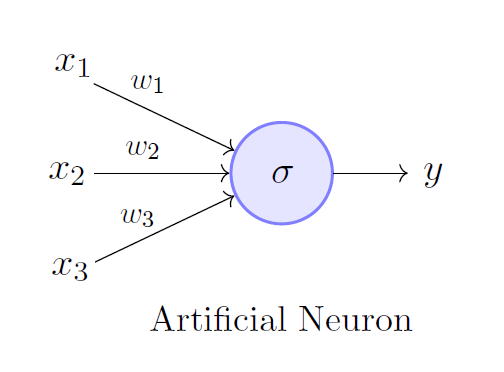
\includegraphics[width=.75\textwidth]{images/perceptron} 
\end{center}
\end{frame}

\begin{frame}
\begin{center}
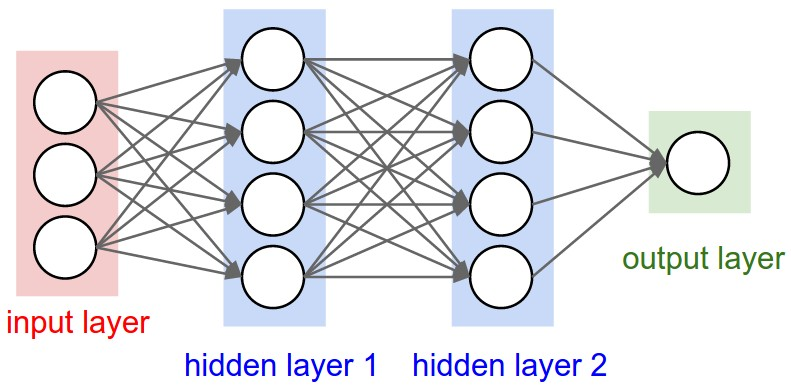
\includegraphics[width=\textwidth]{images/simple_neural_network_header.jpg} 
\end{center}
\end{frame}

\begin{frame}
\begin{center}
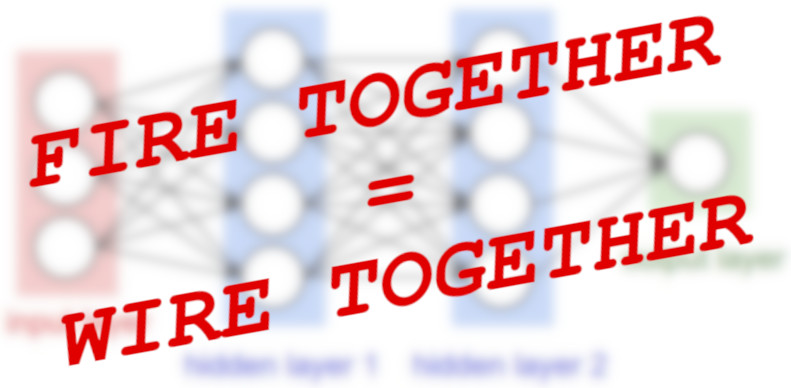
\includegraphics[width=\textwidth]{images/simple_neural_network_header_FW.jpg} 
\end{center}
\end{frame}

%------------------------------------------------------------------------------------

%------------------------------------------------------------------------------------

\section{Die Probleme}

\begin{frame}
\begin{center}
\huge
Where Machine Learning\\ Still Goes Wrong
\end{center}
\end{frame}

\begin{frame}[fragile]

\begin{center}
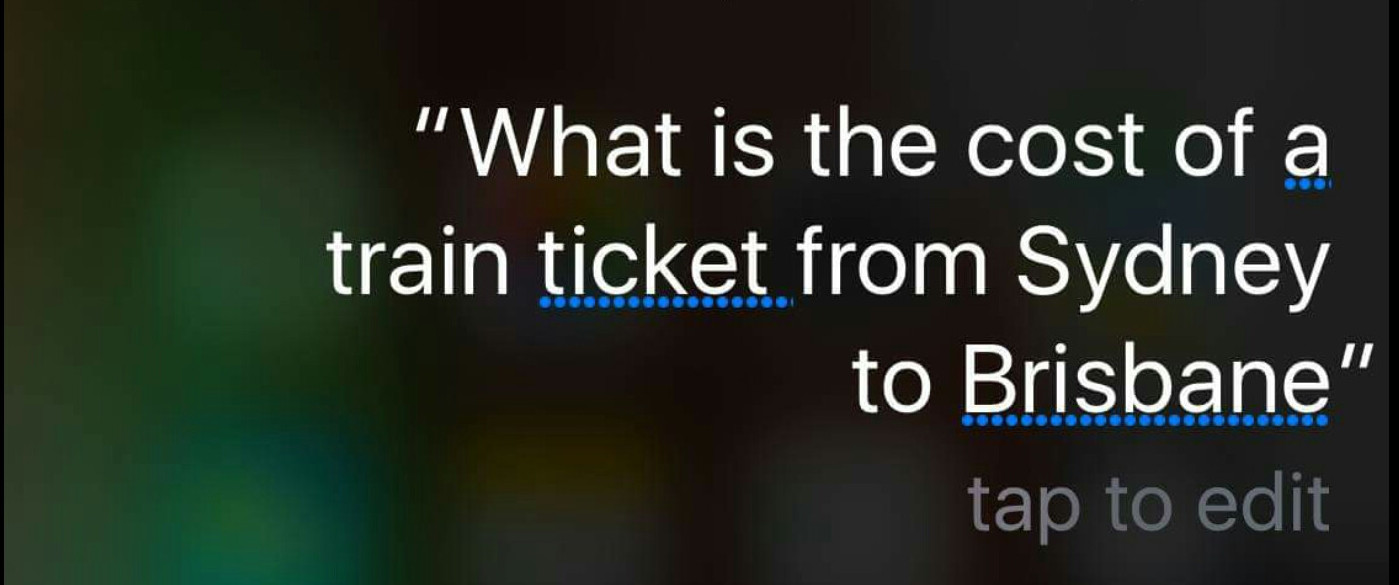
\includegraphics[scale=0.125]{images/sirifail1.jpg} 
\end{center}

\pause
\bigskip

\begin{multicols}{2}

\begin{center}
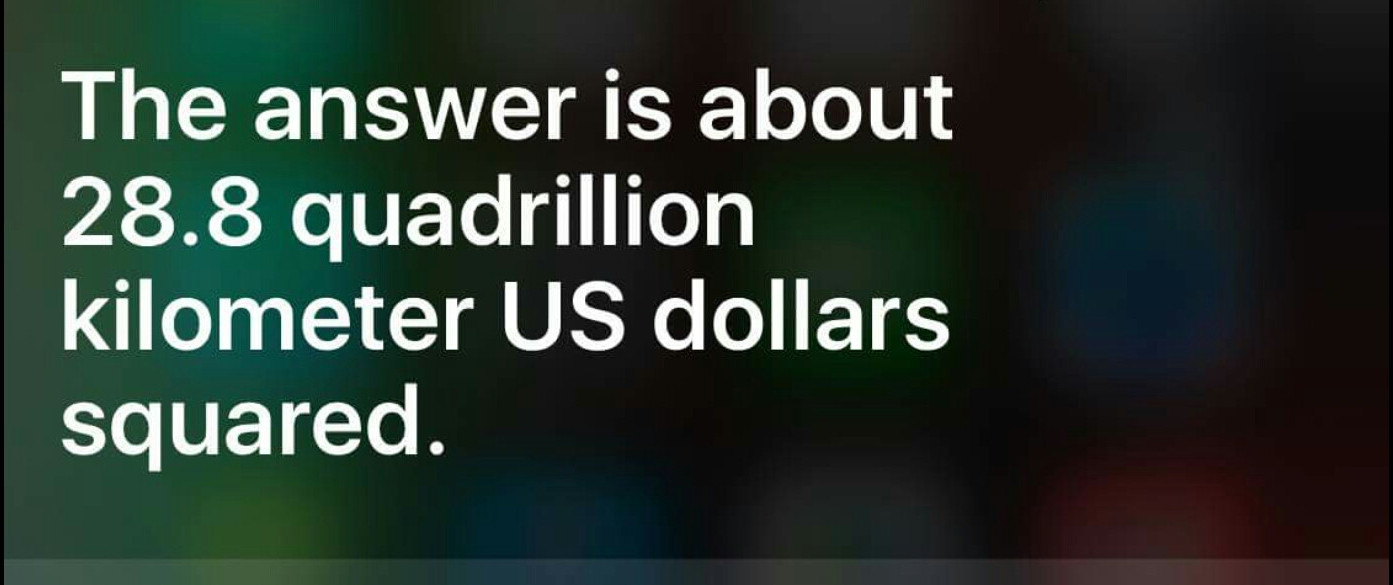
\includegraphics[scale=0.125]{images/sirifail2.jpg} 
\end{center}

\columnbreak
\pause

\begin{center}
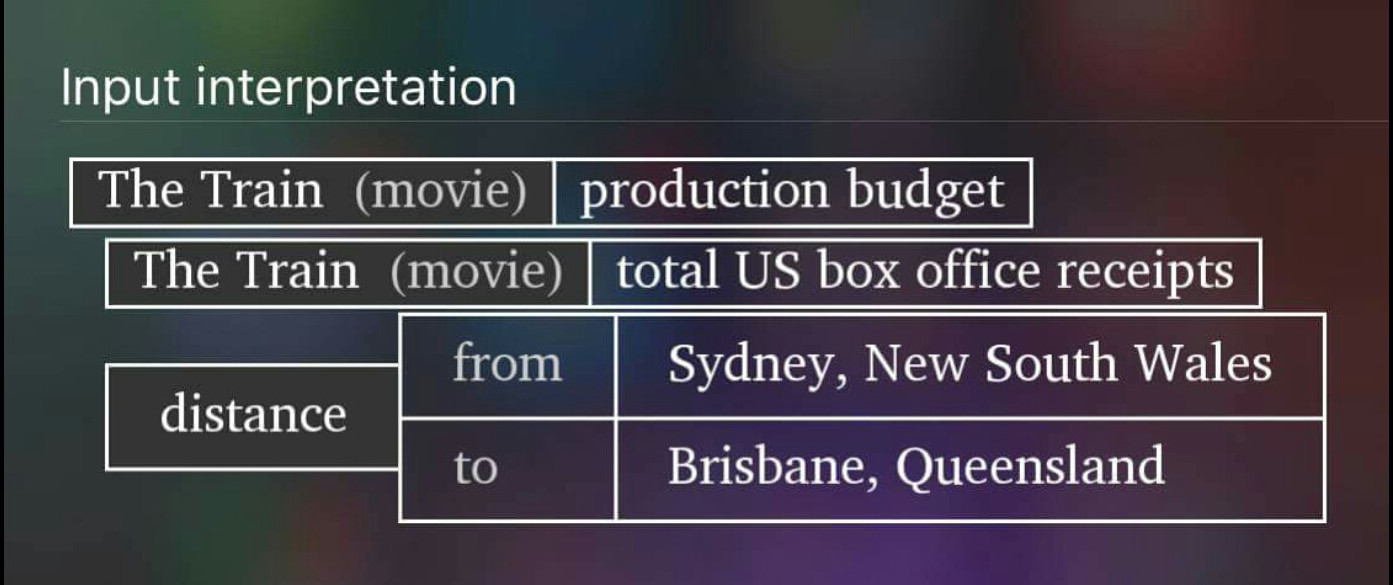
\includegraphics[scale=0.125]{images/sirifail3.jpg} 
\end{center}

\end{multicols}
\end{frame}

\begin{frame}
\begin{center}
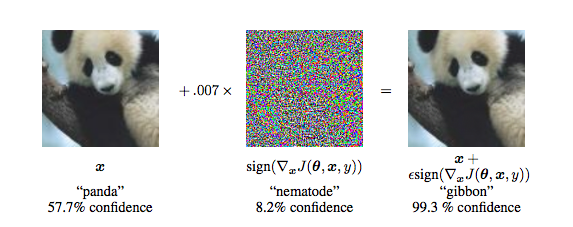
\includegraphics[width=\textwidth,keepaspectratio]{images/recog_panda.png} 
\end{center}
\end{frame}

\begin{frame}
\begin{center}
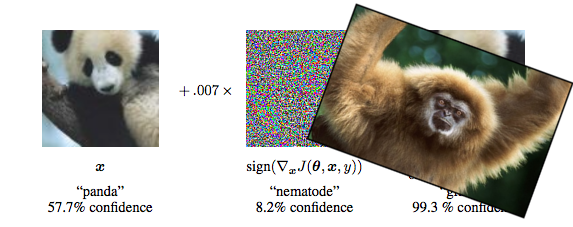
\includegraphics[width=\textwidth, keepaspectratio]{images/recog_gibbon.png} 
\end{center}
\end{frame}


\begin{frame}
\begin{center}

\includegraphics[height=0.65\textheight,keepaspectratio]{images/deep_neural_networks_1.png}
\end{center}
\end{frame}

\begin{frame}
\begin{center}
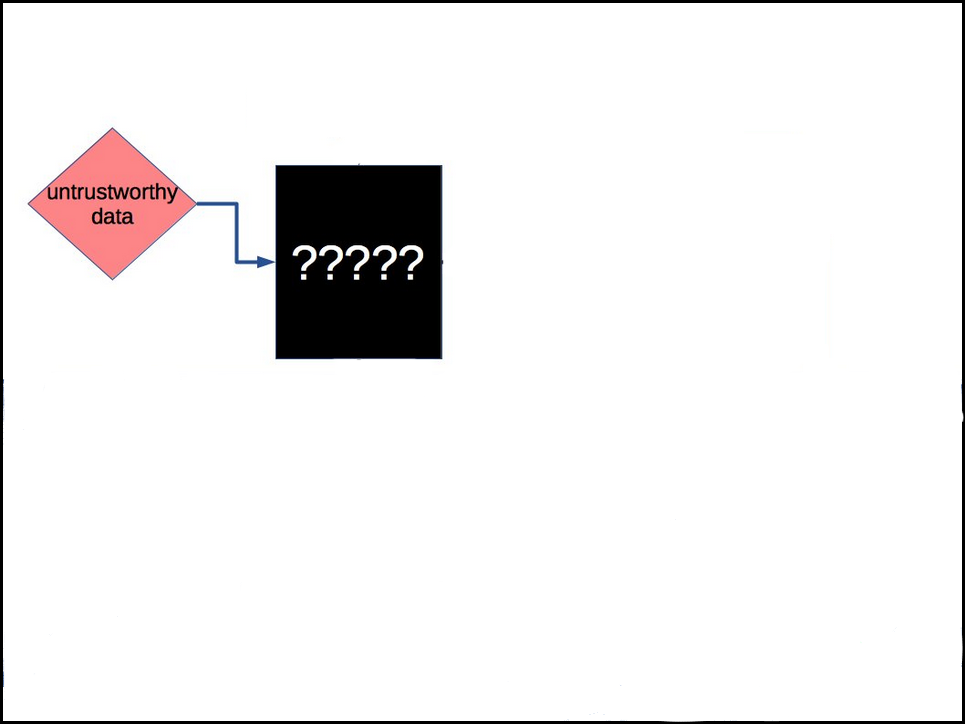
\includegraphics[height=0.65\textheight,keepaspectratio]{images/deep_neural_networks_2.png} 
\end{center}
\end{frame}

\begin{frame}
\begin{center}
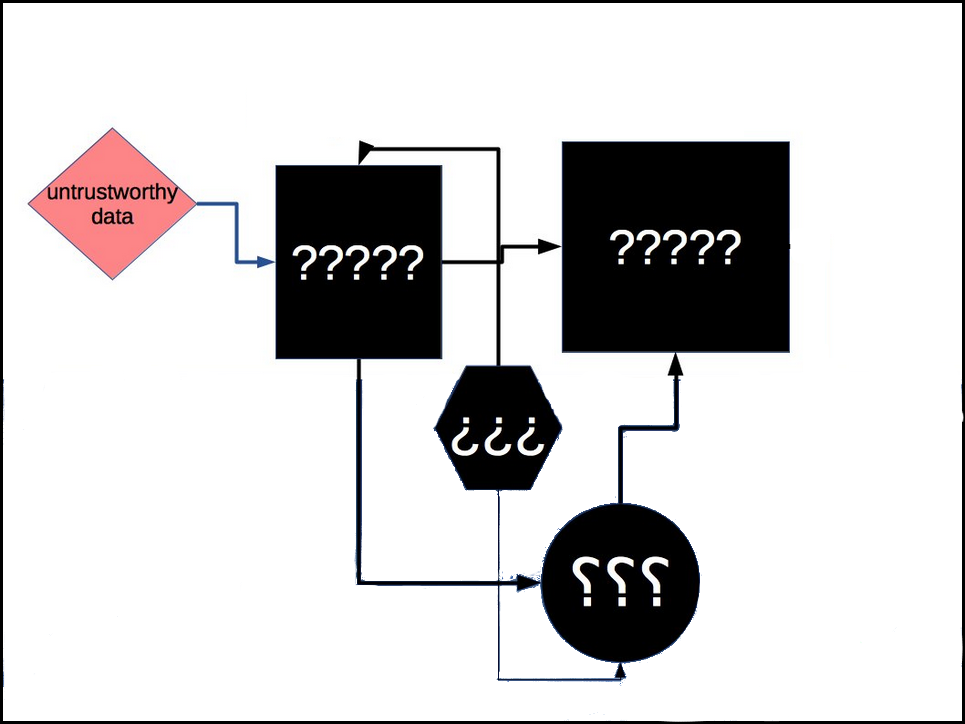
\includegraphics[height=0.65\textheight,keepaspectratio]{images/deep_neural_networks_3.png} 
\end{center}
\end{frame}

\begin{frame}
\begin{center}
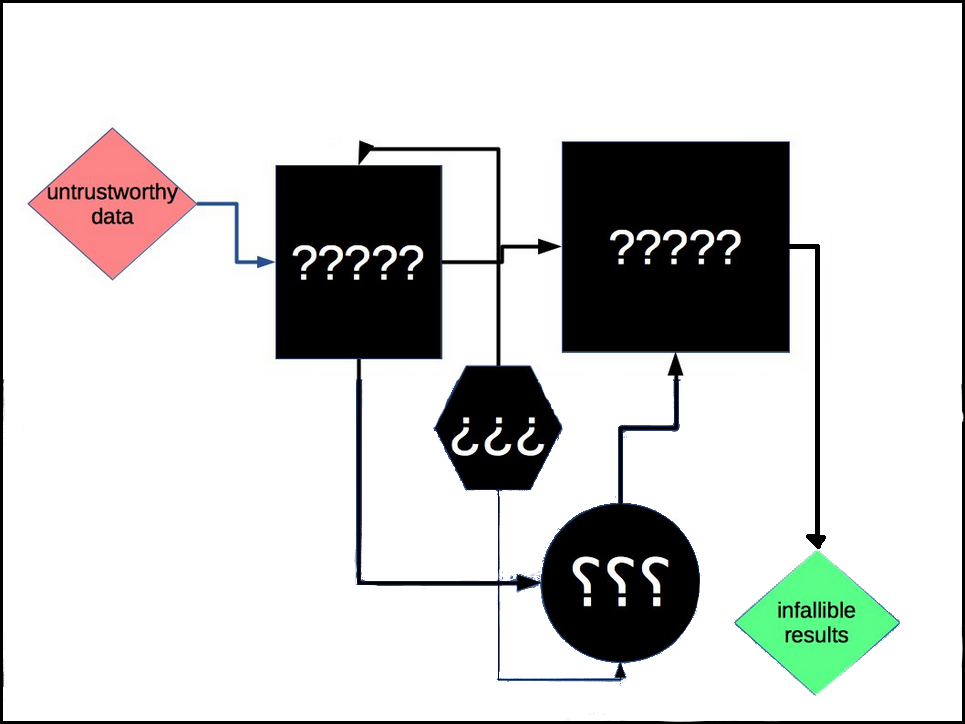
\includegraphics[height=0.65\textheight,keepaspectratio]{images/deep_neural_networks_4.png} 
\end{center}
\end{frame}

%------------------------------------------------------------------------------------

\subsection{Common Problems}

\begin{frame}
\begin{center}
\huge
Practical Problems
\end{center}
\end{frame}

\begin{frame}
\begin{multicols}{2}
\begin{center}
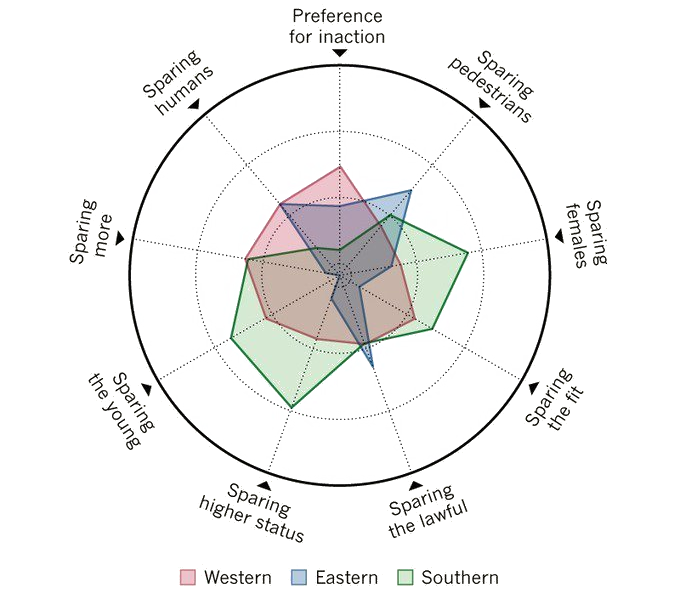
\includegraphics[scale=1.25]{images/morals.png} 
\end{center}
\columnbreak

\begin{center}
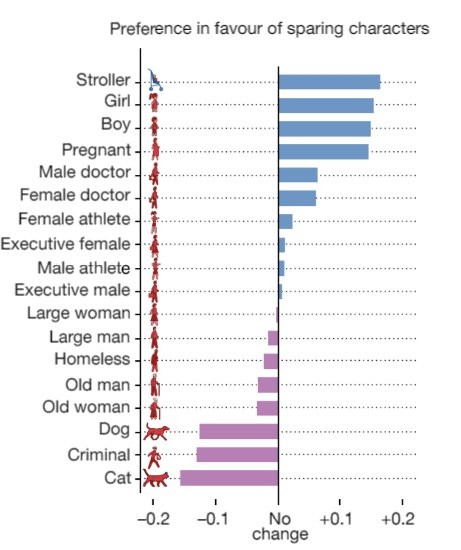
\includegraphics[scale=1.45]{images/sparing} 
\end{center}
\end{multicols}
\end{frame}

%------------------------------------------------------------------------------------

\subsection{Adversarial Objects}
\begin{frame}
\begin{center}
\huge
\glqq Adversarial Objects\grqq
\end{center}
\bigskip
\normalsize

(\textit{Noun, plural}) Objects that seem ordinary to the human eye, but look radically different to image recognition software.
\bigskip

\begin{center}
\textbf{Source:}\\
\emph{Fooling Neural Networks in the Physical World}\\
\url{https://www.labsix.org/}
\end{center}
\end{frame}

\begin{frame}
\begin{center}
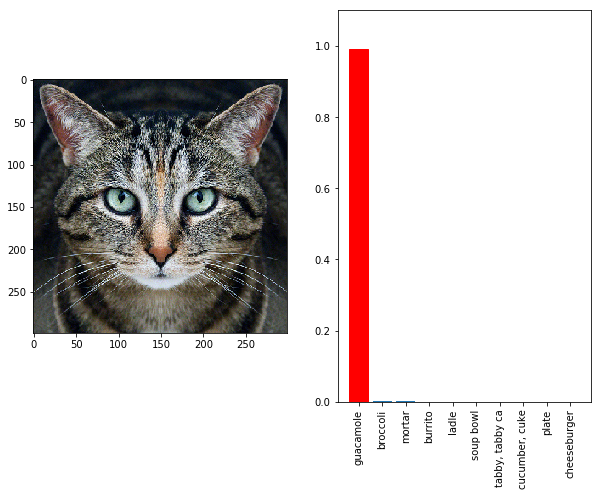
\includegraphics[height=\textheight]{images/cat_adversarial.png} 
\end{center}
\end{frame}

\begin{frame}
\begin{center}
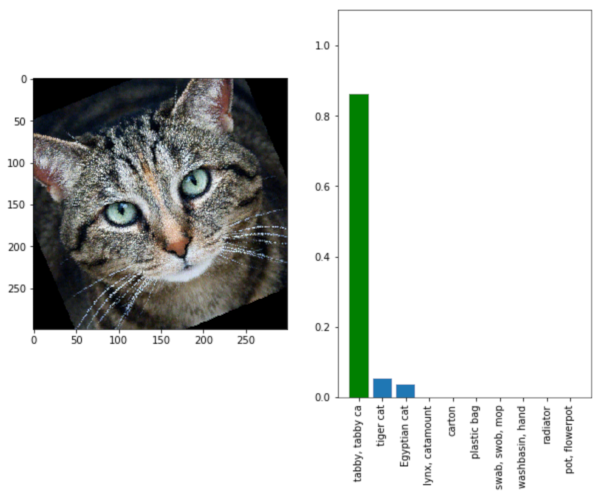
\includegraphics[height=\textheight]{images/cat_rotated.png} 
\end{center}
\end{frame}

\begin{frame}

\begin{center}
Adverserial 3D-printed turtle:
\end{center}

\begin{center}
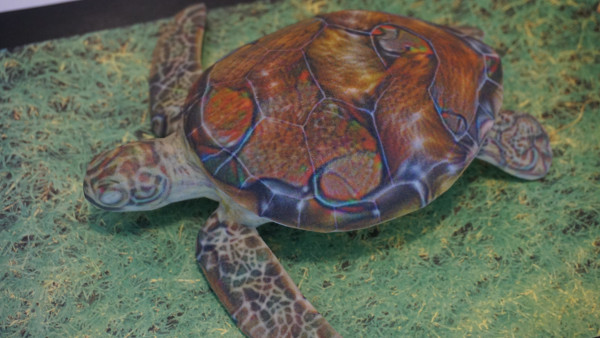
\includegraphics[width=0.8\textwidth]{images/rifle_turtle.jpg} 
\end{center}
\end{frame}

\begin{frame}
\begin{center}
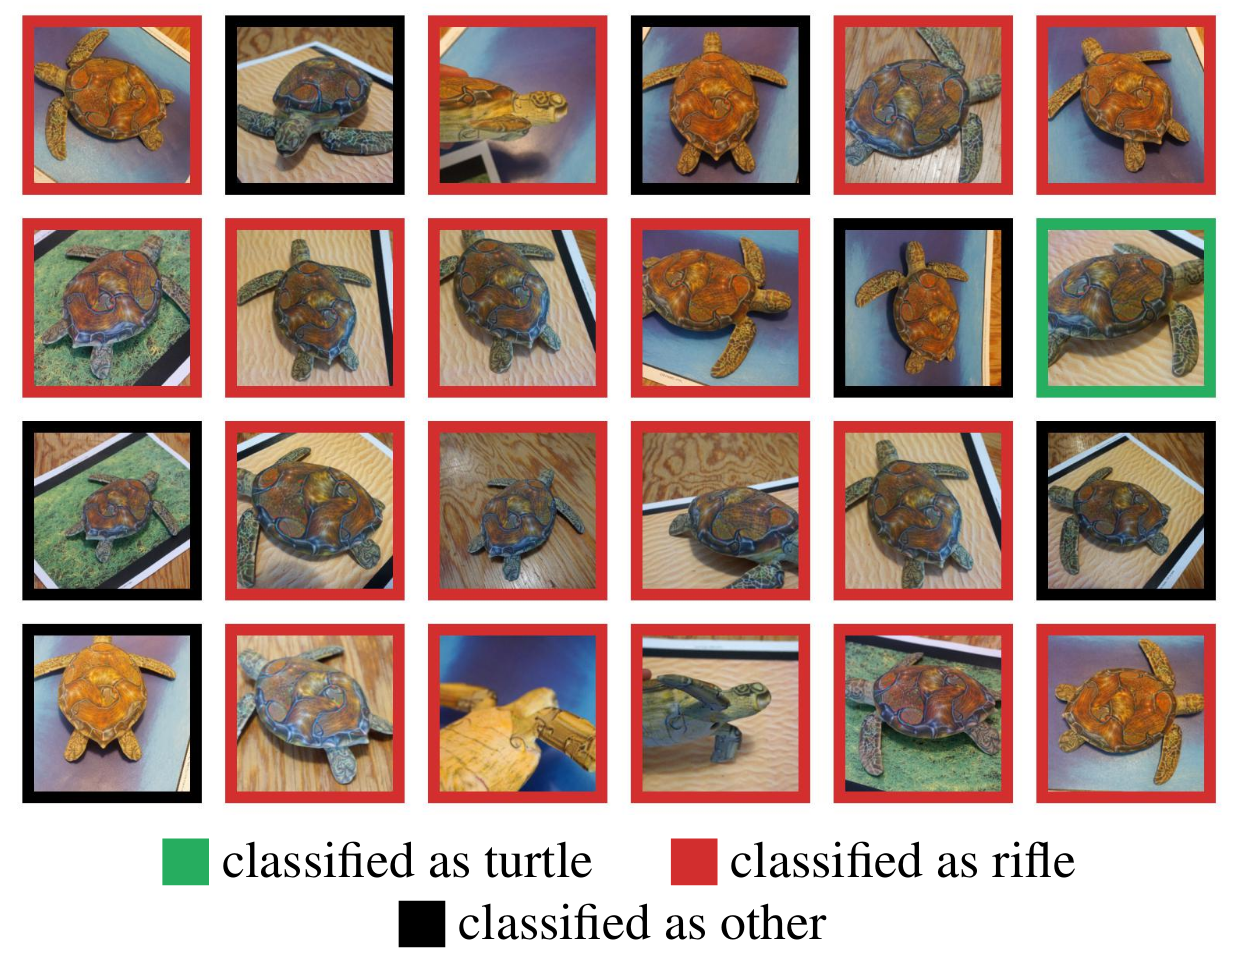
\includegraphics[width=0.7\textwidth]{images/turtle_class} 
\end{center}
\end{frame}

\begin{frame}[fragile]
\begin{multicols}{2}

\vspace*{60pt}
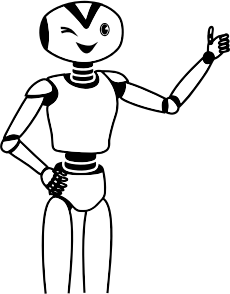
\includegraphics[scale=0.6]{images/Happy-Thumbs-Up-Robot.png} 

\columnbreak

\vspace*{60pt}

\Huge
\hspace*{-30pt}Thank you\\ \hspace*{-20pt} for listening!
\end{multicols}
\end{frame}

\end{document}

